\newcommand\chapternumber{3}
\documentclass[12pt,a4paper]{article}
\usepackage{fullpage}
\usepackage[top=2cm, bottom=4.5cm, left=2.5cm, right=2.5cm]{geometry}
\usepackage{amsmath,amsthm,amsfonts,amssymb,amscd}
\usepackage{lastpage}
% \usepackage{enumitem}
\usepackage{fancyhdr}
\usepackage{mathrsfs}
\usepackage{xcolor}
\usepackage{graphicx}
\usepackage{listings}
\usepackage{hyperref}
\usepackage{tikz}
\usetikzlibrary{shapes,backgrounds}
\usepackage[utf8]{inputenc}
\usepackage[ruled, vlined]{algorithm2e}
% \usepackage{apacite}
\usepackage{csquotes}

% Edit these as appropriate
\newcommand\course{Data Science II}
\newcommand\NetID{sliu1@uvm.edu}
\newcommand\Author{Sida Liu}
\pagestyle{fancyplain}
\headheight 35pt
\lhead{\NetID\\\Author}
\chead{\textbf{\Large \pagetitle }}
\rhead{\course \\ \today}
\lfoot{}
\cfoot{}
\rfoot{\small\thepage}
\headsep 1.5em

\setlength{\parskip}{\baselineskip}%
\setlength{\parindent}{0pt}%

\newenvironment{list_abc}
{ \begin{enumerate}[label=(\alph*)] }
    { \end{enumerate} }

\newenvironment{list_iv}
{ \begin{enumerate}[label=\roman*.] }
    { \end{enumerate} }

\hypersetup{
  colorlinks=true,
  linkcolor=blue,
  filecolor=magenta,
  urlcolor=cyan,
}

\usepackage[overload]{empheq}
\usepackage{tikz}
\usetikzlibrary{bayesnet}
\usetikzlibrary{arrows}

\usepackage{xparse}
\NewDocumentCommand\Cycle{O{} m m m O{} m}{%
% [opt arg cycle]{Node}{Angle}{Node size}[opt arg arch node]{cycle size}
\draw[#1](#2.{#3+asin(#6/(#4*1.41))}) arc (180+#3-45:180+#3-45-270:#6/2) #5;
}

% no color for hyperlinks
\usepackage{hyperref}
\hypersetup{
  colorlinks=true, 
  citecolor=blue, 
  linkcolor=blue, 
  urlcolor=blue
}

\usepackage{enumerate}
\usepackage{float}

\begin{document}
Collaborators: Julia Zimmerman, Jordan Donovan, Sam Rosenblatt, Milo Trujillo, Phil Nguyen, Nicholas Vartanian,Connor Klopfer, Brett Meyer...
We might have discussed problems related to the assignments via Slack.
\section{Manual Gradient Descent}
\begin{align*}
    \frac{\partial \ell_i}{\partial \theta_j} = -2 x_{ij} (y_i - \sum_{j'=1}^{p} x_{ij'} \theta_{j'}) \\
\end{align*}
\begin{align*}
    \nabla_{\theta} \ell & = \sum_{i=1}^{N} \begin{bmatrix}
        \frac{\partial \ell_i}{\partial \theta_1} \\
        \frac{\partial \ell_i}{\partial \theta_2} \\
        \vdots                                    \\
        \frac{\partial \ell_i}{\partial \theta_p} \\
    \end{bmatrix} \\\\
                         & = -2 x^T (y-x\theta)
\end{align*}

I used the dataset this \href{https://www.kaggle.com/sulianova/cardiovascular-disease-dataset}{Cardiovascular Disease dataset}.

The are 70k records in this dataset.
The task is to predict whether a person has cardiovascular disease or not base on his age, height, etc.
I split the dataset into 80\% training and 20\% testing.

The source code is on \href{https://github.com/liusida/ds2/blob/main/assignment3/code/q1.py}{GitHub q1.py}.

I discovered that larger batch size and larger learning rate will result in faster convergence,
however, if learning rate is too large, the learning might diverge,
and if batch size and learning rate is too large will cause overflow.
So I normalized the input to reduce the possibility of overflow, and choose a batch size of 7k, and a small learning rate.
Now the learning process with 1k epochs takes 1.5 seconds. (If I use a batch size of 100, it will take 9.8 seconds.)

The final test accuracy is 0.643.
I also report the final confusion matrix:
Sensitivity 0.574, Specificity 0.712,
Precision 0.667, Negative Predictive Value 0.625.

\begin{figure}[h]
    \centering
    \includegraphics[width=.8\textwidth]{./q1.pdf}
    \caption{Learning curve and two test points.}
\end{figure}

Why would I choose to manually do gradient descent?
Because I want to learn how it works, and also, as David mentioned in class, sometimes we have constraints in practice, for example there's possibility that PyTorch is not supported.

\newpage
\section{2D Rosenbrock function}
\begin{figure}[h]
    \includegraphics[width=.99\textwidth]{./rosenbrock.pdf}
    \caption{Visualization of 2D Rosenbrock function. $x \in (-30,30)$, $y \in (-300,800)$}
\end{figure}

It is hard for SGD because the low area is not a dot but a long belt.
If the learning rate is large, it will diverge.
If the learning rate is low, it will be very slow in finding the minima on that flat belt.

Analytically, we need to solve the equations: $\frac{\partial f}{\partial x} = 0$ and $\frac{\partial f}{\partial y} = 0$.

\begin{align*}[left = \empheqlbrace]
    \frac{\partial}{\partial x} (1-x)^2+100(y-x^2)^2 & = 0 \\
    \frac{\partial}{\partial y} (1-x)^2+100(y-x^2)^2 & = 0 \\
\end{align*}

\begin{align*}[left = \empheqlbrace]
    400x^3-400xy+2x-2 & = 0  \\
    y                 & =x^2 \\
\end{align*}

\begin{align*}
    400x^3-400x^3+2x-2 & = 0 \\
    x                  & =1  \\
    y                  & =1  \\
\end{align*}

Using routine gradient descent, start from $x_0=0, y_0=0$, learning rate $\gamma=10^{-3}$, run for 10k steps.
The optimization successfully converged to the minimum.

This is because the initialization is quite close to the minimum,
and because it is smooth in $x \in (0,1)$ and $ y \in (0,1)$.
Figure \ref{fig:routine_gd} shows the trajectory of the optimization.

\begin{figure}[h]
    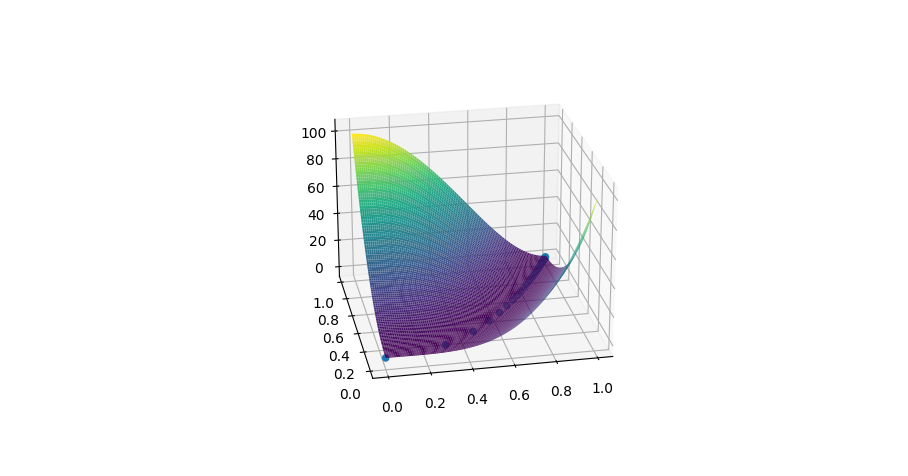
\includegraphics[width=.8\textwidth]{./routine_gd.png}
    \caption{Visualization of the optimization trajectory. $x \in (0,1)$, $y \in (0,1)$.}
    \label{fig:routine_gd}
\end{figure}

If we are not that lucky and use a bad initialization, such as $x_0 = 3$, $y_0 = -2$,
then the routine gradient descent will be harder.
The learning rate need to be smaller, otherwise it will diverge.
Then momentum is needed to speed the optimization up.
I set momentum to 0.99, learning rate $\gamma=10^{-5}$, and run for 10k steps.
The optimization successfully converged to the minimum.
Figure \ref{fig:gd_m} shows the trajectory.

\begin{figure}[h]
    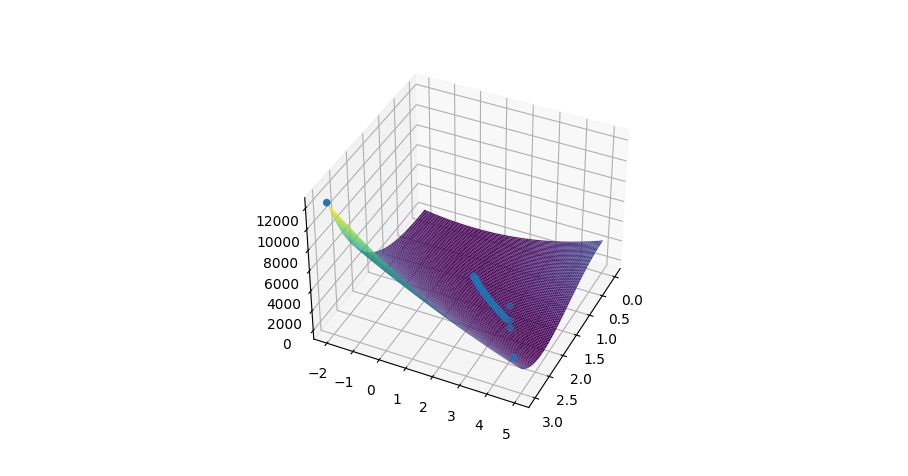
\includegraphics[width=.8\textwidth]{./gd_m.png}
    \caption{Visualization of the optimization trajectory with momentum. $x \in (0,3)$, $y \in (-2,5)$.}
    \label{fig:gd_m}
\end{figure}

The source code is on \href{https://github.com/liusida/ds2/blob/main/assignment3/code/q2.py}{GitHub q2.py}.

\newpage
\section{Math notations and plate notations}
\subsection{Basic Parametric Density Estimation}
Mathematically, let $l=\text{loc}$, $s=\text{inv scale}$, we have:
\begin{align*}
     & p(l, s, d_i)                                                                                                                                                \\
     & \propto p(l)p(s)\prod_{i=1}^N p(d_i|l,s)                                                                                                                    \\
     & = \text{Normal}(0,1) \text{Inv-Gamma}(3,2) \prod_{i=1}^N \text{Normal}(l, s)                                                                                \\
     & = \frac{1}{\sqrt{2\pi}}e^{-\frac{1}{2}l^2} \frac{2^3}{2!}s^{-3-1} e^{-\frac{2}{s}} \prod_{i=1}^N \frac{1}{s\sqrt{2\pi}} e^{-\frac{1}{2}(\frac{d_i-l}{s})^2} \\
     & = 4 (\frac{1}{\sqrt{2\pi}})^{N+1} s^{-4-N} e^{-\frac{l^2}{2} -\frac{2}{s} - \frac{1}{2}\sum_{i=1}^N (\frac{d_i-l}{s})^2}                          \\
\end{align*}
It doesn't seem to have conjugate prior to me.

Plate notation:
\begin{figure}[h]
    \centering
    \tikz{
        % nodes
        \node[obs] (data) {$d_i$};%
        \node[latent,above=of data] (loc) {loc};
        %    \node[latent,above=of loc,xshift=-1cm] (mu) {$\mu$}; %
        %    \node[latent,above=of loc,xshift=1cm] (sigma) {$\sigma$}; %
        \node[latent,left=of data] (scale) {scale};
        \node[latent,left=of scale] (inv_scale) {inv\_scale};
        %    \node[latent,left=of inv_scale,yshift=1cm] (alpha) {$\alpha$};
        %    \node[latent,left=of inv_scale,yshift=-1cm] (beta) {$\beta$};
        % plate
        \plate [inner sep=.3cm,xshift=.02cm,yshift=.2cm] {plate1} {(data)} {N}; %
        % edges
        %    \edge {sigma,mu} {loc}
        %    \edge {alpha,beta} {inv_scale}
        \edge {inv_scale} {scale}
        \edge {scale,loc} {data}
    }
    \caption{Plate notation}
\end{figure}

\newpage
\subsection{Continuous, nonstationary hidden Markov}

Mathematically, let $l=\text{loc}$, $s=e^{\text{log scale}}$, $o=\text{obs scale}$, we have:
\begin{align*}
     & p(l,s,o,x_{n,t},y_{n,t})                                                                                                                                         \\
     & =p(l)p(s)p(o)\prod_{n=1}^N p(x_{n,0}|l,s) \prod_{t=1}^T p(x_{n,t}|l,x_{n,t-1},s) p(y_{n,t}|x_{n,t}, o)                                                           \\
     & =\text{Normal}(0,1) \text{LogNormal}(0,1) \text{Gamma}(2,2) \prod_{n=1}^N \text{Normal}(l,s) \prod_{t=1}^T \text{Normal}(l+x_{n,t-1},s) \text{Normal}(x_{n,t},o) \\
     & =\frac{1}{\sqrt{2\pi}}e^{-\frac{l^2}{2}} \cdot
    \frac{1}{s\sqrt{2\pi}}e^{-\frac{\log(s)^2}{2}} \cdot
    \frac{1}{2!2^2}o^{2-1}e^{-\frac{o}{2}}  \cdot
    \prod_{n=1}^N
    \frac{1}{s\sqrt{2\pi}}e^{-\frac{(x_{n,0}-l)^2}{2s^2}}
    \prod_{t=1}^T
    \frac{1}{s\sqrt{2\pi}}e^{-\frac{(x_{n,t}-l-x_{n,t-1})^2}{2s^2}}
    \frac{1}{o\sqrt{2\pi}}e^{-\frac{(y_{n,t}-x_{n,t})^2}{2o^2}}                                                                                                         \\
\end{align*}

Plate notation (Reference: \href{https://davidrushingdewhurst.com/blog/2020-07-28keep-using-plate-notation.html}{this blog post}):
\begin{figure}[h]
    \centering
    \tikz{
        % \draw[lightgray,ultra thin] (-6,-6) grid (6,6);
        % nodes
        \node[obs] (y_t) {$y_{n,t}$};%
        \node[latent,left=of y_t] (x_t) {$x_{n,t}$};%
        \node[latent,above=of x_t] (x_0) {$x_{n,0}$};%
        \node[latent,above=of x_0,xshift=1.5cm] (loc) {loc};%
        \node[latent,right=of loc] (scale) {scale};%
        \node[latent,above=of scale] (log_scale) {log scale};%
        \node[latent,right=of y_t] (obs_scale) {obs scale};%
        % plate
        \plate [inner sep=.3cm,xshift=.02cm,yshift=.2cm] {episode} {(x_t)(y_t)} {T}; %
        \plate [inner sep=.3cm,xshift=.02cm,yshift=.2cm] {plate1} {(x_0)(episode)} {N}; %
        % edges
        \edge {obs_scale,x_t} {y_t}
        \edge {loc,scale} {x_t}
        \edge {loc,scale} {x_0}
        \edge {log_scale} {scale}
        % hmm...
        \draw[blue, thick, ->,shorten >=1pt] (x_0) to [out=-90,in=90] node[left,yshift=.2cm,xshift=-.2cm] {$t=1$} (x_t);
        \Cycle[blue, ->]{x_t}{180}{7mm}[{node[anchor=0,pos=0.5]{$t=2,...,T (t-1\rightarrow t)$}}]{7mm}
    }
    \caption{Plate notation}
\end{figure}

\newpage
\subsection{Switching model}
Mathematically, let $s'=\text{log scale}$, $s=e^{s'}$, $w=\text{switch}$, $m_1=\text{model1}$, $m_2=\text{model2}$, we have:
\begin{align*}
     & p(s,z_0,z_t,p_t,m_{1,t},m_{2,t},w_{t,n},y_{t,n},x_{t,n})                                                                                             \\\\
     & =p(s)p(z_0|s) \times                                                                                                                                 \\
     & \prod_{t=1}^T p(z_t|z_{t-1}) p(p_t|z_t) 
     \prod_{n=1}^N p(w_{t,n}|p_t) 
     p(m_{1,t}|t) p(m_{2,t}|t) p(y_{t,n}|w_{t,n},m_{1,t},m_{2,t}) 
     p(x_{t,n},y_{t,n}) \\\\
     & =\text{LogNormal}(0,1)
    \text{Normal}(0,s) \times                                                                                                                               \\
     & \prod_{t=1}^T \text{LogitNormal}(z_{t-1},1)
    \prod_{n=1}^N \text{Bernoulli}(p_t)
    p(m_{1,t}|t) p(m_{2,t}|t)
    p(y_{t,n}|w_{t,n},m_{1,t},m_{2,t})
    \text{Poisson}(y_{t,n})                                                                                                                                 \\\\
     & =\frac{1}{s\sqrt{2\pi}}e^{-\frac{\log(x)^2}{2}} \cdot
    \frac{1}{s\sqrt{2\pi}}e^{-\frac{z_0^2}{2s^2}} \cdot \\
    &\prod_{t=1}^T \frac{1}{\sqrt{2\pi}} e^{-\frac{\text{logit}(z_t-z_{t-1})^2}{2}} \cdot
    \prod_{n=1}^N p_t^{w_{t,n}} (1-p_t)^{1-w_{t,n}}
    p(m_{1,t}|t)^{w_{t,n}} p(m_{2,t}|t)^{1-w_{t,n}}
    \frac{y_{t,n}^{x_{t,n}} e^{-y_{t,n}}}{x_{t,n}!}
\end{align*}


Plate notation (next page):
\begin{figure}[!t]
    \centering
    \tikz{
        % \draw[lightgray,ultra thin] (-6,-6) grid (6,6);
        % nodes
        \node[obs] (x_t) {$x_{n,t}$};%
        \node[latent, left=of x_t] (y_t) {$y_{n,t}$};
        \node[latent, below=of y_t, xshift=-2cm] (model1) {model1$_t$};
        \node[latent, below=of y_t] (model2) {model2$_t$};
        \node[latent, left=of y_t, yshift=2cm] (switch) {switch$_{t,n}$};
        \node[latent, left=of switch] (p) {$p_t$};
        \node[latent, left=of p] (z) {$z_t$};
        \node[latent, above=of z] (z0) {$z_0$};
        \node[latent, above=of z0] (scale) {scale};
        \node[latent, left=of scale] (log_scale) {log scale};
        % plate
        \plate [inner sep=.3cm] {plate_switch} {(x_t)(y_t)(switch)} {N};
        \plate [inner sep=.3cm] {episode} {(plate_switch)(model1)(model2)(p)(z)} {T};
        % edges
        \edge {scale} {z0};
        \edge {log_scale} {scale};
        \edge {z} {p};
        \edge {p} {switch};
        \edge {switch, model1, model2} {y_t};
        \edge {y_t} {x_t};
        \draw[blue, thick, ->,shorten >=1pt] (z0) to [out=-90,in=90] node[left,yshift=.2cm,xshift=-.2cm] {$t=1$} (z);
        \Cycle[blue, ->]{z}{180}{7mm}[{node[anchor=0,pos=0.5]{$t=2,...,T (t-1\rightarrow t)$}}]{7mm}
    }
    \caption{Plate notation}
\end{figure}

\newpage
\section{PPL via Pyro}

The source code is on GitHub:
\begin{enumerate}
    \item \href{https://github.com/liusida/ds2/blob/main/assignment3/code/q4.1.py}{q4.1.py}.
    \item \href{https://github.com/liusida/ds2/blob/main/assignment3/code/q4.2.py}{q4.2.py}.
    \item \href{https://github.com/liusida/ds2/blob/main/assignment3/code/q4.3.py}{q4.3.py}.
\end{enumerate}

\newpage
\section{Project Thoughts}
\subsection{Bayesian Learning Signal}
I like Deep Learning.

In Supervised Learning, the learning signal comes from the difference between the truth label $y$ and the prediction $\hat{y}$.

To analyze its assumption, I perform a derivation using MAP:

Suppose we observe a image $\cal{I}$, we want to know a vector representation of the image $h$ that can tell us $y=\text{argmax}(h)$.

Assuming the prior to be $h_0 \sim \textbf{Uniform}(a,b)$, here $a$ and $b$ are constants.
The observation $\hat{h}$ is the representation produced by the network after seeing the image,
Assuming $\hat{h} \sim \textbf{Normal}(h, \sigma)$, here we don't know $\sigma$ yet.
This Normal distribution is saying the network can produce a prediction that is centered at $h$ but very noisy.
These two are quite strong assumptions.

Now I can use MAP to compute the point estimate for $h_0$ given $\hat{h}$:
\begin{align*}
    p(h_0|\hat{h}) &\propto p(\hat{h}|h_0) p(h_0)\\
    &= \textbf{Normal}(h,\sigma) \cdot \textbf{Uniform}(a,b) \\
    &= \frac{1}{\sigma \sqrt{2 \pi}} e^{-\frac{(h-\hat{h})^2}{2\sigma^2}} \cdot 1\\
\end{align*}

Solve $\frac{d}{dh}p(h_0|\hat{h})=0$ to find the maximum:
\begin{align*}
    \frac{h_0-\hat{h}}{\sigma^3} e^{-\cdots} &= 0\\
    h_0-\hat{h} = 0
\end{align*}

So we want to update our belief from $h_0$ to $h_1$: $h_1 = \hat{h}$.

This is how we find the update target, I think?
And we apply L2 loss to it, it'll just like a normal supervised learning signal.

Now if the agent has the chance to observe a very similar image $\cal{I}'$, here we don't use the i.i.d. assumption,
so a better prior should be $h_1$ after the update of the first step.
The problem here is that by using MAP, we only have a point estimator, 
we don't have a distribution for $h_1$, how can I discover a good $h_1$?

Why I am doing this?

Imagine there is a robot with a camera on its face.
It will observe the world, frame by frame.
I assume the current frame of the world is very much similar to the previous frame.
If I can derive a learning signal from this assumption,
the agent will be able to learn without human providing labels.

Once there is a good way to produce the representation $h$ of the image,
we can use whatever existing supervised learning or reinforcement learning to utilize this representation,
and the learning will be faster, I hope.

I read \cite{wang_survey_2020}. It focus of this paper is to connect Bayesian Inference and Deep Learning at an application level, which is not my focus. 
But I learned some basic concepts from it.
The so called Bayesian treatments might give the distribution of $h$.

\subsection{Thought two}

With a second thought, the previous idea turns out to be a Recurrent Neural Network.

The representation $h_t$ is just the hidden state.

\begin{figure}[h]
    \centering
    \includegraphics[width=.8\textwidth]{./rnn.pdf}
    \caption{A RNN with Bayesian updated hidden states.}
\end{figure}

The purpose of the observation is to build a good $h_t$, 
so that if other modules want to use this representation,
it is readily accessible.

So the job for the network module $N$ is to update $h_t$ properly using Bayesian Theorem.

This is different from the Bayesian Neural Networks (BNN).
In BNN, people tries to make the weights and biases to be r.v.'s.

In the Long Short Term Memory (LSTM) model, there is a cell state, which is similar to this $h$.
Maybe replacing this gating and addition with a Bayesian update will give what I want.

\begin{figure}[h]
    \centering
    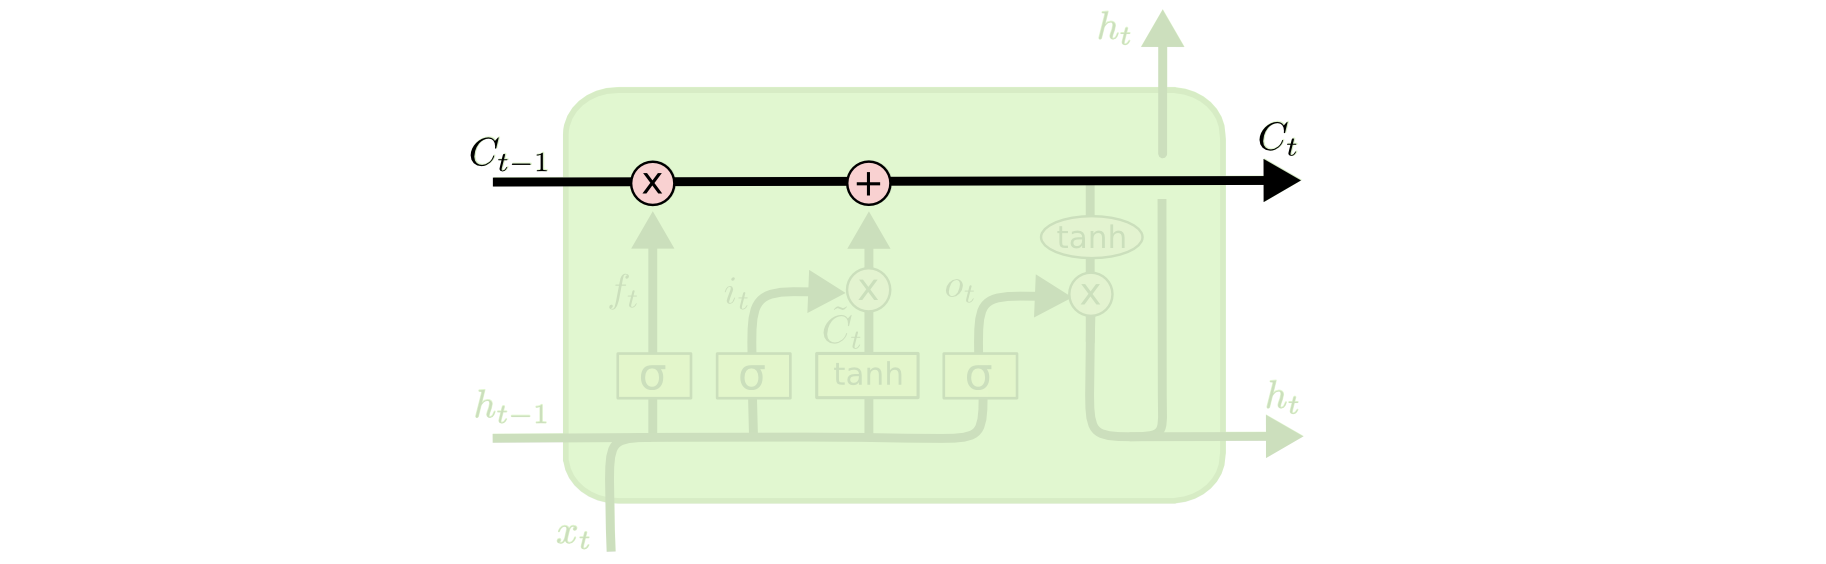
\includegraphics[width=.8\textwidth]{./LSTM3-C-line.png}
    \caption{Cell States are updated by Gating and Addition.}
\end{figure}

Later,
I realized it is related to the World Model  \cite{ha_world_2018},
where they use a variational autoencoder to get a latent $z$ (we call that $h$ earlier), and pass that into a RNN.
However, the $h$ produced by the RNN in the World Model is not parameters of distributions, maybe I can improve this.

\begin{figure}[h]
    \centering
    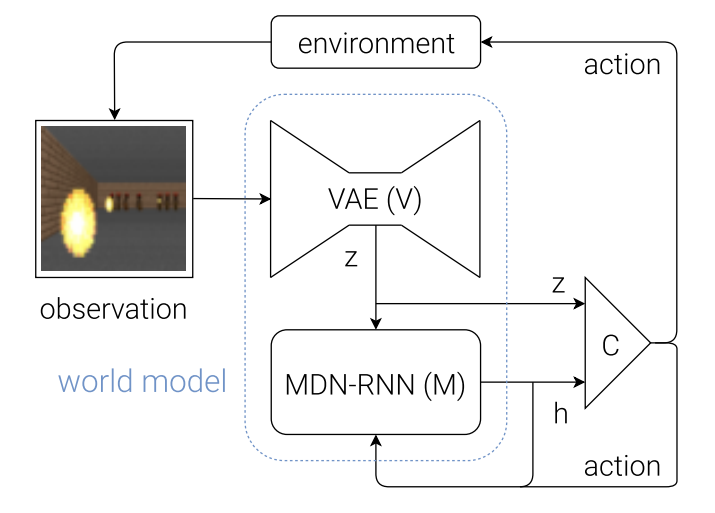
\includegraphics[width=.5\textwidth]{./world_model.png}
    \caption{In the World Model, the $z$ is produced by VAE, so $z$ is the parameters of some distributions.}
\end{figure}



\subsection{Automated Model Search?}

Another thought for the course project is from the idea of automated architecture search.
The architectures are analogous to the generative models in Bayesian Inference.
And people use Evolutionary Algorithms to search for better architectures rather than design it manually \cite{real_regularized_2019}.

So a typically case could be, the EA produces a population of DAGs, 
and BI get all the parameters, and we have a set of final performances,
and EA produces a new population of DAGs by mutating the best DAGs,
and BI get all the parameters again, and we get another set of the performances.

But I am still not familiar with the whole Bayesian Inference process, so I'm not sure if the idea of automated design can be applied to Bayesian Inference.

\bibliographystyle{apalike}
\bibliography{b}

\end{document}
